%% The following is a directive for TeXShop to indicate the main file
%%!TEX root = diss.tex

\chapter{Capacitively coupled double quantum dot}
\label{ch:Methods}

This chapter begins with a discussion of quantum dots in GaAs/AlGaAs as well as discussing some of the relevant energy scales when creating double quantum dot systems. Next, the device used for measurements in this thesis is discussed, and the general measurement protocol is outlined. Finally, results are presented. 


%The focus of this section will be the theory of double (and single) quantum dots in the 2 dimensional electron gas hosted by AlGaAs/GaAs. The basis of this section will be the Fig. \ref{fig:dqd}. In addition, there will be a discussion of the energy scales at play in the system and those that are most important for our entropy measurements.

\section{The device and measurement protocol}
\label{sec:device}

In Ch.~\ref{ch:Theory}, the $\Delta S$ of transition in a potential well from $0 \to 1$ electrons was discussed and it was noted that potential wells like the one described could be built in practice by creating something called a quantum dot. Quantum dots can be built from a wide variety of materials~\cite{bera2010quantum}, and offer a mesoscopic scale realization of something like an ``artifical" atom. For measurements in this thesis, tunable quantum dots are fabricated in a \ac{2DEG} which forms in an AlGaAs/GaAs substrate. In Fig~\ref{fig:qd1} a schematic shows a cross section through such a substrate. When the substrate is cooled to low enough temperature, the bandgap in GaAs and AlGaAs prevents conduction, however, at the interface of the two materials, a sheet of conduction electrons forms which is confined to only two dimension. By adding top gates, as illustrated in Fig~\ref{fig:qd1}, and applying static voltages to these top gates, this sheet of electrons can be further confined to form many structures including quantum dots, quantum wires, and quantum point contacts~\cite{manfra2014molecular}. 
\begin{figure}[h]
\centering
\resizebox{0.7\textwidth}{!}{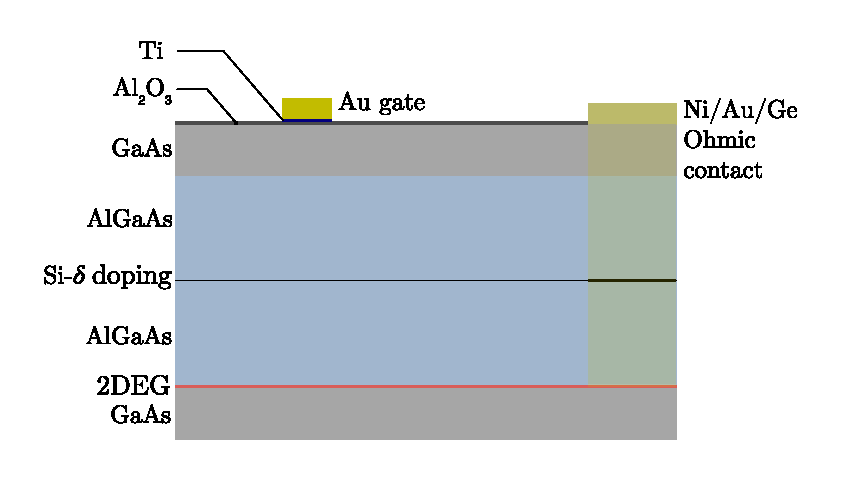
\includegraphics{figures/pdfs/algaas.eps}}
\caption{A cross sectional view of the AlGaAs/GaAs substrate used in measurements for this thesis. A stack of GaAs and AlGaAs forms a \ac{2DEG} at their interface. Ohmic contact is made to the \ac{2DEG} by a thermal annealing process with Ni/Au/Ge further discussed in~\ref{sec:recipes}. Gold (Au) top gates are defined on the surface of the substrate which allow for local control of the density of the \ac{2DEG}.}
\label{fig:qd1}       % Give a unique label to the figure. 
\end{figure}

To study the entropy of a capacitively coupled system, we have fabricated a double quantum dot system in an AlGaAs/GaAs substrate hosting such a \ac{2DEG}. In Fig.~\ref{sec:device}, a top-down image of this device is shown. Two quantum dots are defined, labelled main and impurity dot. 

\begin{figure}[h]
\centering
\resizebox{\textwidth}{!}{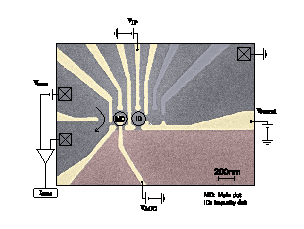
\includegraphics{figures/pdfs/device2.eps}}
\caption{ A top-down SEM image of the device measured in this experiment. Lighter gold regions are the gold gates, while darker regions are the GaAs substrate. A single quantum dot (right hand side) is probed by the leftmost dot whose occupation is measured using $I_{sense}$. In this device, temperature oscillations occur across electrons in a reservoir connected to the probe dot heated via a small thermocurrent through an adjacent quantum point contact. $V_{ACC}$ is used to control the chemical potential, $\mu$, in the probe dot. In the right dot, similar gate structures, labelled $V_{IP}$ allow for the system to be tuned to be tuned degenerate with the probe dot. The X indicates ohmic contact to the 2DEG. The light red section indicates the thermal reservoir of the system. Greyed out gates were not used in this experiment.}
\label{fig:device}       % Give a unique label to the figure. 
\end{figure}


In practice, to measure the entropy of this system using the integral from Eqn.~\ref{eqn:MR} we have a few requirements. First, we assumed constant pressure in the Maxwell relation. In the context of a \ac{2DEG} with which our measurements are conducted, the dominating pressure at temperatures below the Fermi temperature, $T_F \approx 100$K is the degeneracy pressure~\cite{ashcroftmermin}, an incompressibility emerging from the Pauli exclusion principle disallowing fermions from occupying the same quantum state. In addition, by keeping energy fluctuations due to thermal energy, $k_bT$, much smaller than the spacing between energy levels in the dot, we ensure that random temperature fluctuations do not produce unpredictable energy level occupation.

In addition, the primary requirement for using Eqn.~\ref{eqn:MRintegral} is the ability to measure occupation of the system as a function of chemical potential while varying temperature. In this device, the occupation of the main dot is the only measured quantity\footnote{See Sec.~\ref{sec:artifacts}}. We measure $N$ of the main quantum dot by measuring the current $I_{sense}$ through a charge sensing \ac{QPC} seen in Fig.~\ref{fig:device}. Because of the proximity of this \ac{QPC}, referred to as the charge sensor, to the main dot very small electrostatic changes in the main dot affect the conduction across the charge sensor~\cite{spintocharge}. As such, a larger $I_{sense}$ indicates fewer electrons in the main dot, while a smaller $I_{sense}$ indicates more electrons in the main dot. In effect, this means that $I_{sense}$ can be used to directly measure the occupancy of the dot as a function of various other quantities like chemical potential, $\mu$, or temperature, $T$. We use $V_{ACC}$ shown in in Fig.~\ref{fig:device} to locally control the chemical potential of the dot. Varying the electrostatic potential applied to this gate $V_{ACC}$ - and by extension the chemical potential in the dot - is our primary technique to control the occupancy of the dot. Based on this protocol, we can decompose Eqn.~\ref{eqn:MRintegral} into the following quantities which can be determined experimentally.
\begin{equation}
	\label{eqn:eqn2}
	\Delta S = - \int_{\mu_1}^{\mu_2} \frac{dN}{dI_{sense}} \frac{dI_{sense}}{dT} \,\,  d \mu
\end{equation}

This integral tells us that we can measure the change in entropy between two chemical potentials in the dot by measuring two quantities: $dN/dI_{sense}$, and $dI_{sense}/dT$ as a function of chemical potential. The first quantity, $dN/dI_{sense}$ is just a scaling factor that can be independently experimentally determined and does not depend on $\mu$. In fact, $dN/dI_{sense}$ simply represents the current amplitude of a transition from $N \to N+1$ electrons in the dot. The final quantity $dI_{sense}/dT$ does depend on $\mu$ and so must be measured as $\mu$ is changed. Intuitively, $dI_{sense}/dT$ is a measure of the difference between the occupancy of the dot at higher $T$ and lower $T$ times a scaling factor $\delta T$ representing the change in temperature.\footnote{See Sec.~\ref{sec:electrontemp} for a more in depth consideration of $\delta T$ in gate voltage.} This difference between hot and cold curves is illustrated by the shading on the plots in Fig.~\ref{fig:num_int}. 
\begin{figure}[h]
\centering
\resizebox{1\textwidth}{!}{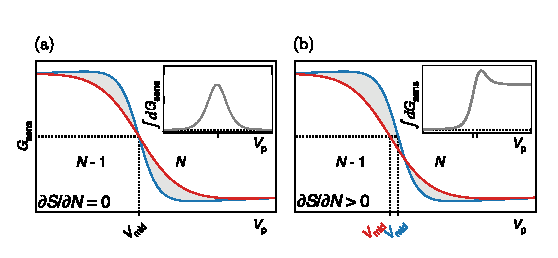
\includegraphics{figures/pdfs/numerical_integrated.eps}}
\caption{In (a) and (b) we show two examples of the measurement protocol where the occupancy of the probe dot is measured using $I_{sense}$. In each case, the occupancy is swept from $N - 1$ to $N$ electrons both at a higher temperature (red) and a lower temperature (blue), however in (a) this change in $N$ does not correspond to an entropy change in the system whereas in (b) we see a positive change in entropy of the system due to this change in occupancy. The inlaid plots show the cumulative integral of $d I_{sense}$ -- or the difference between hot and cold $I_{sense}$ curves. The entropy change of the system is measured by the value of this integral after the completion of this transition. Figure adapted from ~\cite{nikentropy}.}
\label{fig:num_int}       % Give a unique label to the figure. 
\end{figure}

In previous work in the group, Hartman et al.~\cite{nikentropy} used a very similar process except harnessing Eqn.~\ref{eqn:dndt} which allows for $dI_{sense}/dT$ to be fit directly so long as the lineshape of the transition is dominated by thermal broadening in the Fermi distribution of the reservoir. Continued work has focussed on extending the single dot findings to less ideal regimes using Eqn~\ref{eqn:eqn2}~\cite{child2020entropy}. However, the remainder of the results and discussion will focus on measurements of entropy in a double quantum dot system.

\section{Entropy of a double quantum dot system}
\label{sec:dqd}

In Fig.~\ref{fig:device}, a second quantum dot, labelled impurity dot is shown to the right of the main dot. The occupation of this impurity dot can be tuned by changing the potential on $V_{IP}$, effectively changing the chemical potential of the dot. Although the charge sensing \ac{QPC} is farther from this second impurity quantum dot, small changes in $I_{sense}$ can still be detected when the occupation of the impurity dot changes. In Fig.~\ref{fig:qdpanel2} the states of the combined system are mapped out by plotting $dI_{sense}/dV_{IP}$ which changes abruptly when occupation shifts occur in either of the dots. The states are labelled by [occupation of main dot, occupation of impurity dot]. Using these transitions, the states of both dots are mapped out over a wide range of gate voltages in Fig.~\ref{fig:qdpanel2} (a), then zoomed in on the 10, 01 crossing in (b).

\begin{figure}[h]
\centering
\resizebox{1\textwidth}{!}{\includegraphics{figures/pdfs/QD_panel2.eps}}
\caption{In (a) the states of the double quantum dot system are mapped out by charge sensing the occupation of both dots. The color indicates the derivative of the current through the charge sensor. Sudden changes in this current indicate state changes in the two dots, with larger changes (seen as darker on this plot) indicating changes in the main dot, and smaller changes (slightly lighter on this plot) indicating changes in states in the impurity dot. The large squares indicate regions of constant state in the two dots and are labelled by [occupation main dot, occupation impurity dot]. In (b), a zoomed in view on the crossing (white circle in plot (a)) of the $0 \to 1$ transitions in the two dots is shown.}
\label{fig:qdpanel2}       % Give a unique label to the figure. 
\end{figure}

In Fig.~\ref{fig:qdpanel2} (b), the vertical line jagged indicates a transition in the main dot. Along this transition (as $V_{IP}$ changes) one can consider the change in entropy of the entire system as the main dot transitions from $0 \to 1$ electrons shown in Table~\ref{tbl:entropy} (neglecting charge degeneracy).
\begin{center}
	\begin{tabular}{ |c|c|c| } 
		\hline
		Transition & $\Delta S_{sys}$ [$k_B$] & $\Delta S_{main}$ [$k_B$]  \\ \hline\hline
		$00 \to 10$ & $\ln 2$ & $\ln 2$ \\ 
		$01 \to 10$ & 0       & $\ln 2$ \\ 
		$01 \to 11$ & $\ln 2$ & $\ln 2$ \\ 
		\hline
		\end{tabular}
		\captionof{table}{Entropy along 01, 10 transition}\label{tbl:entropy}
\end{center}
Notably, anywhere along this transition, the change in entropy if one considers the main dot only will be $\Delta S = k_B \ln 2$ since it is always transitioning from a no-occupancy state with no spin degeneracy to a single electron state with a spin degeneracy of two. However, in the case of the $01 \to 10$ transition, the finite capacitive coupling between the dots causes the impurity dot to be pushed from occupied to unoccupied as the main dot goes from unoccupied to occupied. This implies a clear discrepancy between $\Delta S_{sys}$ and $\Delta S_{main}$ which will clearly indicate if this protocol continues to work, experimentally, for capacitively coupled systems.

In the case where the impurity dot is tuned to a sufficiently strong tunnel coupling to the reservoir, $\Gamma_{imp}$, that the charge degeneracy during the transition is suppressed, the $\Delta S$ matches the predicted values for $\Delta S_{sys}$ in Table~\ref{tbl:entropy}. This is shown in Fig.~\ref{fig:largeg} where over the course of the transition, $\Delta S$ goes from $k_B \ln 2$ to 0 then back to $k_B \ln 2$.
\begin{figure}[h]
\centering
\resizebox{1\textwidth}{!}{\includegraphics{figures/pdfs/large_gamma_full_figure.eps}}
\caption{Entropy along the 0,1 $\to$ 1,0 transition in the pair of dots with $\Gamma_{main}/T < 1 < \Gamma_{imp}/T$. In (a) the dark region indicates the transition in the main quantum dot. Double dot states are labelled as [Occupation main dot, occupation impurity dot]. The $\Delta S$ of the transition in the main dot is plotted for the double dot transition crossing. In the 0,0 $\to$ 1,0 regime, the $\Delta S$ is found to be roughly $\ln 2 \approx 0.69$ as expected from the spin degeneracy in the probe dot. In the central regime, where there is a full 0,1 $\to$ 1,0 transition, entropy is found to be around $\ln 2 - \ln2 = 0$ since the spin degeneracy of the impurity dot is simply replaced by the spin degeneracy in the probe dot. In (b) the $\Delta I$ between the cold and hot curves plotted in (c) are shown. In (c) the shift in $V_{mid}$ between 70 mK and 50 mK traces can clearly be seen to vary depending on $\Delta S$.}
\label{fig:largeg}        
\end{figure}

In effect, this shows exactly what is expected since thermodynamically, it should not matter what component of the system is being measured if the entire system is undergoing a transition. Another way to understand this is by Fig.~\ref{fig:largeg} (c) which shows the transition in occupation of the main dot at various points in the double dot state digram (a). Each is plotted with both a warm transition and a cold transition. Qualitatively, it is easy to see the relative shift between 50 and 70 mK data like in Fig.~\ref{fig:potential_wells} in the top (purple) transition, however in the center (green) transition, this shift is absent. Although all three transitions are only measurements on the main dot and so are nearly identical regardless of the occupation or change in occupation of the impurity dot, they represent very different state transitions in the system. In the top plot, \textit{only} the main quantum dot is undergoing a transition, whereas in the center plot the larger system is undergoing a transition $01 \to 10$. Although this larger state transition is not detectable in the $N(\mu)$ curve or as it is collected experimentally, the $I_{sense} (V_{ACC})$ signal, it is clear in the $dN/dT$ signal. 

Data was also collected in the case that the impurity dot is less strong coupled to the reservoir, or $\Gamma_{imp}/T < 1$, shown in Fig.~\ref{fig:smallg}. In this case, charge degeneracy in the impurity dot becomes accessible allowing for states with degeneracy of 3 when the impurity dot is between occupied and unoccupied, and also spin degenerate. In this case, one should theoretically expect to see a $\Delta S_{sys} = \ln 2 - ln 3 \approx -0.4$ and a $\Delta S_{sys} = \ln3 \approx 1.1$. In Fig.~\ref{fig:smallg} (b), theoretical predictions are plotted on top of the experimental data, showing approximate agreement. It is believed the disagreement originates from back action noise affects, which are further summarized in Sec.~\ref{sec:back}.

\begin{figure}[h]
\centering
\resizebox{1\textwidth}{!}{\includegraphics{figures/pdfs/small_gamma_full_figure.eps}}
\caption{Entropy along the 0,1 $\to$ 1,0 transition in the pair of dots with $\Gamma_{main}/T \approx \Gamma_{imp}/T < 1$. In (a), $dI_{sense}/dV_{ACC}$ indicates the state of both dots as a function of $V_{IP}$. In (b), theoretical calculations of $\Delta S$ are plotted along with the experimental values, error bars showing 95\% confidence interval. In (c) $dN/dT$ in units of $dI_{sense}/dT$ is plotted.}
\label{fig:smallg}      
\end{figure}


\section{Conclusion}
\label{sec:conclusion}

Not yet sure what the focus of this section will be, still thinking about it.




\endinput

Any text after an \endinput is ignored.
You could put scraps here or things in progress.
